\chapter{Options-Implied Features}
\label{ch:options-implied}

Layer~2 adds nine features extracted from the SPX implied volatility surface.
These are the first forward-looking inputs in the pipeline: they embed market expectations about future variance that backward-looking RV measures cannot capture.

%% ──────────────────────────────────────────────
\section{Features}
\label{sec:implied-features}
%% ──────────────────────────────────────────────

\begin{table}[htbp]
\centering
\caption{Layer~2 feature set: options-implied features from the SPX surface.}
\label{tab:implied-features}
\small
\begin{tabular}{%
  >{\raggedright\arraybackslash}p{3.0cm}
  >{\raggedright\arraybackslash}p{6.2cm}
  >{\raggedright\arraybackslash}p{3.0cm}}
\toprule
\textbf{Feature} & \textbf{What It Is} & \textbf{Horizon Impact} \\
\midrule
ATM IV (30-day) &
  Average of 50-delta put and call IVs from Marquee ERDVOL surface: $\IVol_t^{\mathrm{ATM}} = \tfrac{1}{2}\bigl(\sigma_{50\Delta P} + \sigma_{50\Delta C}\bigr)$ &
  All horizons \citep{GuKellyXiu2020} \\[8pt]
VRP &
  $\VRP_t = (\IVol_t^{\mathrm{ATM}})^2 - \E_t[\RV_{t+1:t+22}]$, estimated using HAR forecast as the RV expectation &
  1w--1m strongest \citep{BTZ2009} \\[8pt]
25-Delta Risk Reversal &
  $\mathrm{RR}_t = \sigma_{25\Delta C} - \sigma_{25\Delta P}$; measures skew demand for downside protection &
  1--5d \\[8pt]
Term Structure Slope &
  $\mathrm{TS}_t = \IVol_t^{3\mathrm{m}} - \IVol_t^{1\mathrm{m}}$; positive in calm markets, inverts pre-crisis &
  1w--1m \\[8pt]
Butterfly &
  $\mathrm{BF}_t = \sigma_{25\Delta P} + \sigma_{25\Delta C} - 2\,\IVol_t^{\mathrm{ATM}}$; measures tail thickness beyond skew &
  Crisis detection \\[8pt]
VVIX &
  $\VVIX_t$: implied volatility of VIX options; vol-of-vol signal &
  1--5d \\[8pt]
VIX Term Structure &
  $\mathrm{VTS}_t = F_t^{3\mathrm{m}} / \mathrm{VIX}_t$; ratio $> 1$ = contango (calm), $< 1$ = backwardation (stress) &
  Regime signal \\[8pt]
IV--RV Gap &
  $\mathrm{Gap}_t = \IVol_t^{\mathrm{ATM}} - \sqrt{\RV_t^{(m)} \times 252}$; residual risk premium beyond VRP &
  1--5d \\[8pt]
Event-Implied Vol &
  Extracted from the surface around known event dates (FOMC, earnings); isolates the vol the market attributes to the event &
  Pre-event only \\
\bottomrule
\end{tabular}
\end{table}


%% ──────────────────────────────────────────────
\section{Horizon Dependence}
\label{sec:horizon-dependence}
%% ──────────────────────────────────────────────

Options-implied features contribute almost nothing at $h = 1$ but become the dominant source of marginal improvement at weekly and monthly horizons.
Figure~\ref{fig:options-horizon} summarizes the pattern.

\begin{figure}[htbp]
\centering
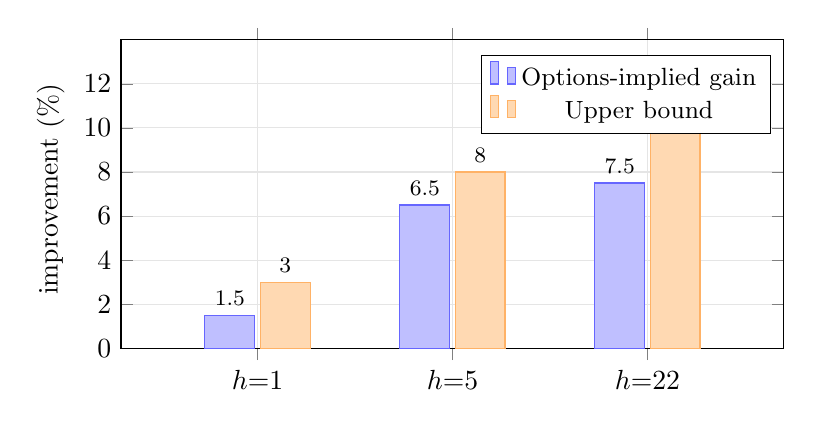
\begin{tikzpicture}
\begin{axis}[
  ybar,
  width=10cm,
  height=5.5cm,
  bar width=18pt,
  ylabel={$\QLIKE$ improvement (\%)},
  symbolic x coords={$h{=}1$, $h{=}5$, $h{=}22$},
  xtick=data,
  ymin=0, ymax=14,
  ytick={0, 2, 4, 6, 8, 10, 12},
  nodes near coords,
  nodes near coords align={vertical},
  every node near coord/.append style={font=\footnotesize},
  enlarge x limits=0.35,
  legend style={at={(0.98,0.95)}, anchor=north east, font=\small},
  grid=major,
  grid style={gray!20},
]
\addplot[fill=blue!25, draw=blue!60] coordinates
  {($h{=}1$, 1.5) ($h{=}5$, 6.5) ($h{=}22$, 7.5)};
\addlegendentry{Options-implied gain}

\addplot[fill=orange!30, draw=orange!60] coordinates
  {($h{=}1$, 3.0) ($h{=}5$, 8.0) ($h{=}22$, 10.0)};
\addlegendentry{Upper bound}
\end{axis}
\end{tikzpicture}
\caption{$\QLIKE$ improvement from adding Layer~2 options features on top of Layers~0--1, by forecast horizon. Ranges: $h{=}1$: 1--3\%; $h{=}5$: 5--8\%; $h{=}22$: 5--10\%. Based on literature benchmarks.}
\label{fig:options-horizon}
\end{figure}

The mechanism is straightforward.
At $h = 1$, yesterday's RV is an excellent predictor of tomorrow's RV because volatility is persistent; options add little incremental information.
At $h = 5$ and $h = 22$, the daily signal decays, and the forward-looking content of options prices fills the gap.
Options embed expectations about scheduled events (FOMC, earnings, CPI) that backward-looking RV cannot see.


%% ──────────────────────────────────────────────
\section{What We Compute}
\label{sec:what-we-compute}
%% ──────────────────────────────────────────────

The full SPX IV surface is sourced from Marquee \texttt{ERDVOL\_PERCENT\_STANDARD}.
This provides a complete tenor $\times$ delta grid from which all nine features are extracted.

The surface covers SPX only.
For individual equities, the options-implied features serve as market-wide regime signals (shared across all names in the universe), not stock-specific predictors.
This is consistent with the constraint noted in Chapter~2: no single-name IV surfaces are available.


%% ──────────────────────────────────────────────
\section{Cumulative Performance}
\label{sec:cumulative-performance}
%% ──────────────────────────────────────────────

With Layers~0--2 complete (HAR core, asymmetry/jumps, options-implied), the feature set contains approximately 20 features and captures roughly 85\% of the forecasting accuracy achievable with the full 120-feature pipeline.
The remaining layers (microstructure, cross-asset, engineered interactions) provide diminishing marginal gains.


%% ──────────────────────────────────────────────
%% Boxes
%% ──────────────────────────────────────────────

\begin{keyidea}[ML Advantage Grows with Horizon]
At $h = 1$, HAR ties ML on $\QLIKE$.
At $h = 5$ and $h = 22$, ML models with options-implied features deliver 10--20\% $\QLIKE$ improvement over the best linear baseline.
The advantage comes from nonlinear interactions between VRP, skew, and term structure that linear models cannot capture \citep{ChristensenSiggaardVeliyev2023}.
\end{keyidea}

\begin{warning}[VRP Requires a Realized Variance Forecast]
The VRP is defined as $(\IVol)^2 - \E[\RV]$.
The second term is itself a model output (typically HAR).
Using VRP as an input feature creates a recursive dependency: the VRP feature quality depends on the baseline forecast quality.
Use a simple, fixed HAR estimate for the RV expectation term, not the model being trained.
\end{warning}
